% Harus dimuat terlebih dahulu, digunakan agar file PDF memiliki format karakter yang benar.
% Untuk informasi lebih lanjut, lihat https://ctan.org/pkg/cmap.
\RequirePackage{cmap}

% Format dokumen sebagai paper konferensi menggunakan aturan IEEEtran terbaru (v1.8b).
% Untuk informasi lebih lanjut, lihat http://www.michaelshell.org/tex/ieeetran/.
\documentclass[conference]{IEEEtran}[2015/08/26]

% Format encoding font dan input menjadi 8-bit UTF-8.
\usepackage[T1]{fontenc}
\usepackage[utf8]{inputenc}

% Format bahasa menjadi bahasa german dan inggris.
% \usepackage[indonesian]{babel}
\usepackage[english]{babel}

% Digunakan untuk tujuan demonstrasi.
\usepackage{mwe}

% Digunakan untuk menampilkan font dengan style yang lebih baik.
\usepackage[zerostyle=b,scaled=.75]{newtxtt}

% Digunakan untuk menampilkan tabel dengan style yang lebih baik.
\usepackage{booktabs}

% Digunakan untuk menampilkan gambar pada dokumen.
\usepackage{graphicx}

% Digunakan untuk menampilkan potongan kode.
\usepackage{listings}
\lstset{
  basicstyle=\ttfamily,
  columns=fixed,
  basewidth=.5em,
  xleftmargin=0.5cm,
  captionpos=b
}

% Digunakan agar backticks (`) dapat dirender pada PDF.
% Untuk informasi lebih lanjut, lihat https://tex.stackexchange.com/a/341057/9075.
\usepackage{upquote}

% Digunakan untuk menyeimbangkan bagian akhir dokumen dengan dua kolom.
\usepackage{balance}

% Digunakan untuk menampilkan pustaka.
\usepackage[square,comma,numbers,sort&compress]{natbib}

% Mengubah format ukuran teks pada natbib.
\renewcommand{\bibfont}{\normalfont\footnotesize}

% Menambah nama penulis ketika menggunakan perintah \citet.
% Untuk informasi lebih lanjut, lihat https://tex.stackexchange.com/a/76075/9075.
\usepackage{etoolbox}
\makeatletter
\patchcmd{\NAT@test}{\else \NAT@nm}{\else \NAT@hyper@{\NAT@nm}}{}{}
\makeatother

% Digunakan untuk melakukan linewrap pada pustaka dengan url yang panjang
% jika terdapat hyphens
\usepackage[hyphens]{url}

% Digunakan untuk menambah hyperlink pada referensi.
\usepackage{hyperref}

% Menonaktifkan warna dan bookmark pada hyperref.
\hypersetup{hidelinks,
  colorlinks=true,
  allcolors=black,
  pdfstartview=Fit,
  breaklinks=true
}

% Digunakan untuk membenarkan hyperref pada gambar.
\usepackage[all]{hypcap}

% Digunakan untuk menampilkan beberapa gambar
\usepackage[caption=false,font=footnotesize]{subfig}

\usepackage{stfloats}

% Tambahkan format tanda hubung yang benar di sini
\hyphenation{
  ro-ket
  me-ngem-bang-kan
  per-hi-tu-ngan
  tech-ni-ques
}

\begin{document}

  % Ubah kalimat berikut sesuai dengan judul penelitian.
\title{Mimicking Between Humanoid Robot and Human Based on Real-Time Pose Estimation}

% Ubah kalimat-kalimat berikut sesuai dengan nama, institusi, alamat dan kontak penulis.
\author{
  \IEEEauthorblockN{Nathanael Hutama Harsono}
  \IEEEauthorblockA{Department of Computer Engineering\\
    Faculty of Intelligent Electrical\\
    and Informatics Technology\\
    Sepuluh Nopember Institute\\
    of Technology\\
    Surabaya, Indonesia 60111\\
    nathanael.19072@mhs.its.ac.id}

  \and
  \IEEEauthorblockN{Mauridhi Hery Purnomo}
  \IEEEauthorblockA{Department of Computer Engineering\\
    Faculty of Intelligent Electrical\\
    and Informatics Technology\\
    Sepuluh Nopember Institute\\
    of Technology\\
    Surabaya, Indonesia 60111\\
    hery@ee.its.ac.id}

  \and
  \IEEEauthorblockN{Dion Hayu Fandiantoro}
  \IEEEauthorblockA{Department of Computer Engineering\\
    Faculty of Intelligent Electrical\\
    and Informatics Technology\\
    Sepuluh Nopember Institute\\
    of Technology\\
    Surabaya, Indonesia 60111\\
    dion@its.ac.id}
  
  \and
  \IEEEauthorblockN{\centerline{Muhtadin}}
  \IEEEauthorblockA{Department of Computer Engineering\\
    Faculty of Intelligent Electrical\\
    and Informatics Technology\\
    Sepuluh Nopember Institute\\
    of Technology\\
    Surabaya, Indonesia 60111\\
    muhtadin@te.its.ac.id}
}

% Digunakan untuk menampilkan judul dan deskripsi penulis.
\maketitle

  % Mengubah keterangan `Abstract` ke bahasa indonesia.
% Hapus bagian ini untuk mengembalikan ke format awal.
\renewcommand\abstractname{Abstact}

\begin{abstract}

  % Ubah paragraf berikut sesuai dengan abstrak dari penelitian.
  The habit of doing regular physical activity is a central protective factor for health.
  However, sometimes the motivation to engage in physical activity decreases with age.
  Luckily, this can be overcome by replacing the position of a physical trainer with a humanoid robot.
  The main difference between this study and some previous studies is comparing humanoid robot's pose with human's pose directly, 
  which will be used in the process of mimicking of robots to humans.
  The main program in this study will be divided into 2 parts: RECORD and PLAY modes. In RECORD mode, human will do some poses and robot will imitate them
  while saving the movement. Whereas in PLAY mode, the robot will move according to the movements that have been stored in the previous mode and humans will imitate the robot's movements (the robot acts as a trainer).
  Then an assessment of human movement will be carried out based on robot movement using cosine similarity and the results will be obtained in percentage form.
  The greater the value, the more similar human pose and robot pose are, and vice versa.
  By using MediaPipe Pose for keypoint estimation in humans and RCNN Keypoint for robots, the created system is able to provide an accurate assessment of the similarity between the 2 poses.

\end{abstract}

% Mengubah keterangan `Index terms` ke bahasa indonesia.
% Hapus bagian ini untuk mengembalikan ke format awal.
\renewcommand\IEEEkeywordsname{Index Terms}

\begin{IEEEkeywords}

  % Ubah kata-kata berikut sesuai dengan kata kunci dari penelitian.
  Cosine Similarity, Mimicking, Physical activity.

\end{IEEEkeywords}


  % Ubah bagian berikut sesuai dengan konten-konten yang akan dimasukkan pada dokumen
  % Ubah judul dan label berikut sesuai dengan yang diinginkan.
\section{Introduction}
\label{sec:introduction}

% Ubah paragraf-paragraf pada bagian ini sesuai dengan yang diinginkan.

Robots have experienced significant development over the last few years 
because of their ability to perform multiple tasks quickly and precisely.
One form of development is socially assistive robots (SARs). 
SARs are a type of robot that combines the aspects of assistive robotics (AR)
and socially interactive robotics (SIR), so it makes SARs a robot capable of providing assistance to users in the form of social interaction \citep{feil2005}.

Regular physical activity is a central protective factor for health.
A report from WHO says that lack of physical activity contributes to around 3.2 million premature deaths each year worldwide.
The research also shows that regular exercise can help older adults improve physical fitness, immune system, sleep quality, stress levels, and overcome other health problems \citep{lotfi2018}.
However, motivation to engage in physical activity declines with age. 
This is due to understaffed and high costs of personal trainers as well as the elderly who cannot be permanently motivated and instructed to engage in physical activity.
Based on research conducted by \citet{ruf2020} it can be concluded that the use of humanoid robot can motivate older people to carry out regular physical activity.

The application of SARs is very diverse, for example, humanoid robot that become physical trainers for children \citep{güneysu2017}, 
robotic systems for physical training of the elderly \citep{avioz2021}, and so on. The methods used also vary, for instance, 
you can put sensors on the user and get feedback, then provide a response based on the data obtained through the sensor \citep{güneysu2017}. 
Another method is to use pose estimation obtained through \emph{deep learning} models.
However, previous studies have only compared the angle and depth of each keypoint from estimated human pose within certain boundaries or compared the results of human poses with the poses that are used as a guide \citep{romeo}.
There is still little study that directly compares the suitability between poses performed by human and robot.

For that, on this occasion, we propose study related to mimicking between humanoid robot and human based on real-time pose estimation. 
In addition to finding the best pose estimation method for both humanoid robot and human, this study will also compare poses between them and make a web for controlling their interaction.

Pembahasan pada paper ini dimulai dengan presentasi mengenai penelitian lain (Bagian \ref{sec:relatedworks}).
Kemudian dilanjutkan dengan penjelasan mengenai arsitektur dari sistem yang dibuat (Bagian \ref{sec:poseestimation}).
Berdasarkan hal tersebut, kami menunjukkan lorem ipsum (Bagian \ref{sec:systemdesign}).
Terakhir, didapatkan kesimpulan dari penelitian yang telah dilakukan (Bagian \ref{sec:kesimpulan}).

  % Ubah judul dan label berikut sesuai dengan yang diinginkan.
\section{Related Works}
\label{sec:relatedworks}

% Ubah paragraf-paragraf pada bagian ini sesuai dengan yang diinginkan.

Previous studies have succeeded in creating a model that can obtain multi-robot pose estimation from images.
This research was conducted by \citet{amini2021} from the University of Bonn using the bottom-up approach method.
The bottom-up approach is a method that detects body joints and groups them into individuals simultaneously.
However, the dataset that used only for adult-size category robots and a few for robots without skin. Therefore,
we will add data from the Ichiro robot, where the Ichiro robot is a robot category teen size and type of robot without skin.

In addition, as done by \citet{güneysu2017} who developed an assistive robot as a physical trainer for young children.
They have designed and implemented a fully autonomous human-robot interaction system with social assistance that can increase a
child's involvement in a variety of physical exercise by providing real-time feedback that they get from the IMU (Inertial Measurement Units) worn on the child.
However, in contrast to previous research, this research does not use any sensors that are worn by the user. This will most likely increase users' convenience during physical exercise.
  % % Ubah judul dan label berikut sesuai dengan yang diinginkan.
% \section{Pose Estimation}
% \label{sec:poseestimation}

% % Ubah paragraf-paragraf pada bagian ini sesuai dengan yang diinginkan.

% \subsection{Pose Estimation}
% \label{subsec:poseestimation}

% Pose estimation is a heavily explored area with applications in gaming, animation, action recognition, activity tracking, and augmented reality.
% In order to improve pose estimate outcomes, various approaches have been developed. These methods may generally be split into: single-person and multi-person approaches.
% The single-person approach is fundamentally a regression issue because it just determines the pose of a single person in an image, 
% the person's position and an implicit number of keypoints are already known. However, the multi-person approach tries to solve an unconstrained problem because we do not know 
% the positions and number of persons within the image, therefore the framework has to detect keypoints and assemble an unknown number of persons \citep{romeo}.

% \subsection{Human and Humanoid Robot Pose Estimation}
% \label{subsec:uhmanandrobotposeestimation}

% Pose estimation on humans can be divided into two techniques: 2D Pose Estimation and 3D Pose Estimation.
% 2D pose estimation is a type of pose estimation that can estimate the locations of the body joints in 2D space relative to input data (i.e., image or video frame). 
% The location is represented in \emph{x, y} coordinates for each key point. On the other hand, 3D pose estimation transforms a 2D image into a 3D object by estimating an additional Z-dimension to the prediction.
% 3D pose estimation enables us to predict the accurate spatial positioning of a represented person or thing.
% Humanoid robots and persons have similar shapes, which has both advantages and disadvantages. On the one hand, this allows us to start with approaches already in use for persons,
% but on the other, it makes it harder for us to distinguish between persons and humanoid robots \citep{amini2021}.
  % Ubah judul dan label berikut sesuai dengan yang diinginkan.
\section{System Design}
\label{sec:systemdesign}

\begin{figure*}[ht]
  \centering
  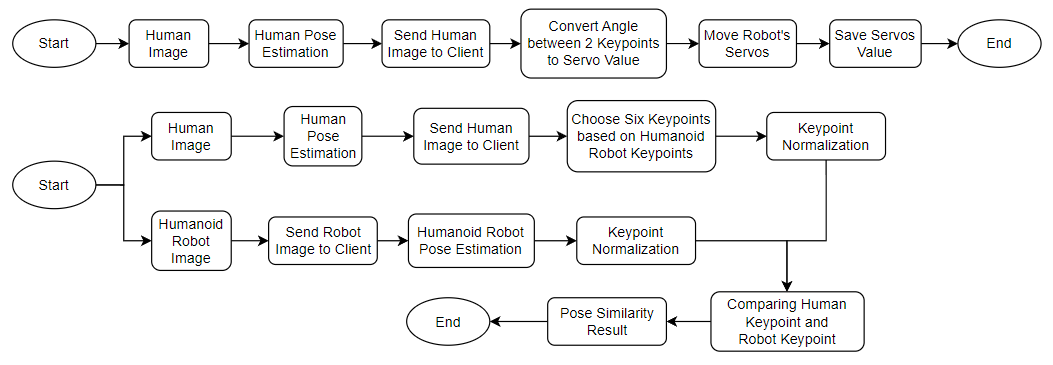
\includegraphics[width=0.95\textwidth]{gambar/methodology.png}
  \caption{Block Diagram of Workflow.}
  \label{fig:block-diagram}
\end{figure*}

As seen in Figure \ref{fig:block-diagram}, the system will be divided into two parts: RECORD (upper) and PLAY mode (bottom).


\subsection{Input Image}
\label{subsec:input-image}

The input image that is fed into both models (human and humanoid robot) is 640x480 pixels with RGB channels. The device for getting the image is the Logitech C920 Webcam. We use OpenCV library to open the camera and capture the image.


\subsection{Human Pose Estimation}
\label{subsec:human-pose-estimation}

Since there are already many pose estimation models for humans out there, we do not need to retrain them and just compare them to find the best model. In order to compare the models, we selected a paper for reference.
So evaluation metrics based on paper and real detection results will be shown in Section \ref{sec:result-and-discussion}, for inference time, we will try in NUC i5. The models that we compare include OpenPose, MediaPipe, and YOLO-pose.
The input for these models is an RGB image and the output is the location of human keypoints.


\subsection{Send Image to Client}
\label{subsec:send-image-to-client}

Our program uses websites to interact with users, the website view can be seen in Figure \ref{fig:websiteview}. There is a Javascript client and a Python Server that communicate via \emph{socketio}.
The server will send human image to the client so we can adjust our position in the camera. This is done to enable the robot to capture the entire human pose.
\begin{figure}[ht]
  \centering
  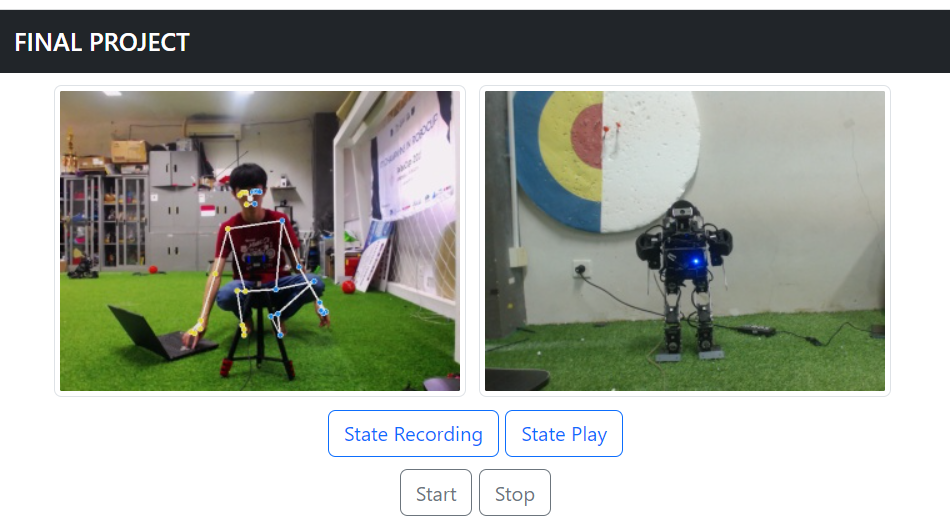
\includegraphics[width=0.48\textwidth]{gambar/web.png}
  \caption{Website View.}
  \label{fig:websiteview}
\end{figure}
The main program is divided into two modes, RECORD mode and PLAY mode. In RECORD mode, a human as a trainer gives a series of movements and will be followed by a humanoid robot, as well as robot saves these movements to use in PLAY mode later.
Meanwhile, in the PLAY mode, the robot acts as a trainer and performs a series of movements according to the movements previously stored in RECORD mode. Human will follow the robot's movement while the robot is also saving both human and robot images and comparing them later. After getting human's keypoint, the server will visualize the detection result and send it as a buffer to the client.


\subsection{Convert Angle to Servo Value}
\label{subsec:convert-angle-to-servo-value}

To be able to move a robot's upper body like human movement, we need to obtain the angle between 2 keypoints using the \emph{arc tangent} function with the input \emph{\{x,y\}} coordinate as shown in Equation \ref{eq:arctan}.
\begin{equation}
  \label{eq:arctan}
  angle = \arctan \left(\frac{Y_2 - Y_1}{X_2 - X_1}\right)
\end{equation}

There are four angles we want to retrieve which are the angles from the shoulder to the elbow (right and left) and also the elbow to wrist (right and left) in order to robot can mimic upper body human movement.
If we look at MediaPipe Pose Landmark, 6 keypoints that become our concern are 11, 12 for shoulders, 13, 14 for elbows, 15, and 16 for wrists. 
We get the right shoulder and left shoulder values by entering landmarks 14, 12, and 13, 11 respectively. 
It is slightly different to obtain the elbow angles because we want its angle to be relative to the shoulder angle by subtracting its angle from the shoulder angle. We also apply limitations for each angle to keep the servo safe as seen in Table \ref{tb:robot-servos}.

\begin{table}
  \caption{Robot Servos Limitations.}
  \centering
      \begin{tabular}{{ccc}}
      \hline
      \rowcolor[HTML]{C0C0C0}
      \textbf{Joint Angle} & \textbf{Motion} & \textbf{Range (deg)} \\
      \hline
      LShoulderRoll       & Left shoulder joint right and left    & -110 to 30  \\
      RShoulderRoll       & Right shoulder joint right and left   & -30 to 110 \\
      LElbowPitch           & Left Elbow joint front and back       & -120 to 10  \\
      RElbowPitch           & Left Elbow joint front and back       & -10 to 120  \\
      \hline
      \end{tabular}
      \label{tb:robot-servos}
  \end{table}


  \subsection{Move Robot's Servos}
  \label{subsec:move-robot-servo}

  ROS2 is used to move the robot's servos.
  On this occasion, we divide the task to move the robot's servo into 2 packages. The first one is named \emph{motion matching} where angle conversion to servo value happen, the other one is \emph{tachimawari},
  a package that provides a DYNAMIXEL's joints management library for a ROS 2 project. Every package has a node with the package's name like Figure \ref{fig:relation-node-record-mode}.
  \begin{figure}[ht]
    \centering
    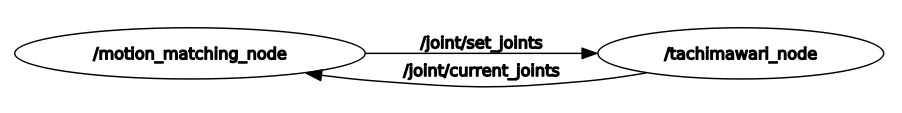
\includegraphics[width=0.48\textwidth]{gambar/rqt_without_akushon.png}
    \caption{Relationship Between Nodes in RECORD Mode.}
    \label{fig:relation-node-record-mode}
  \end{figure}
  Each node communicates with each other through a topic. There are 2 topics in RECORD mode, which are \verb|joint/set_joints| and \verb|joint/current_joints|. 
  After getting desired servos angle from the previous section, we just need to publish it to \emph{tachimawari} node and it will move the servos. 

  In \verb|tachimawari_node| there is \verb|joint_node| that publishes the current joints every 8ms (it is used in the following section) and has a subscriber that listens to joints that we want to move. 
  In order to move servos to the value that we want, we must enable the torque of all servos first. Then we make a command in array form that contains the servo's id and our desired value or target value (16 bytes) that split into 2 * 8 bytes.

\subsection{Save Servos Value}
\label{subsec:save-servo-value}

In the previous section, we discussed a little about the publisher in \emph{tachimawari} package that publishes the value of every current joint of the robot through a \verb|joint/current_joints| topic.
There is also a subscriber in \verb|motion_matching| node that is retrieved that data and a ROS2 timer that is triggered every 0.5 seconds to save the current joints in a JSON format so our robot can move according to the movements exemplified by humans.


\subsection{Humanoid Robot Pose Estimation}
\label{subsec:humanoid-robot-pose-estimation}

In PLAY mode, the server side sends two images so that we can know and adjust the position of humans and robots in the camera. Due to the large network delay when sending two 320x240 pixel images, when the START button is pressed,
the server does not send the image to client again, the robot plays a series of moves stored in the previous JSON file by communicating via another ROS2 packages, while saving both images. After that, when the STOP button is pressed, the server starts to compare poses between them.
\begin{figure}[ht]
  \centering
  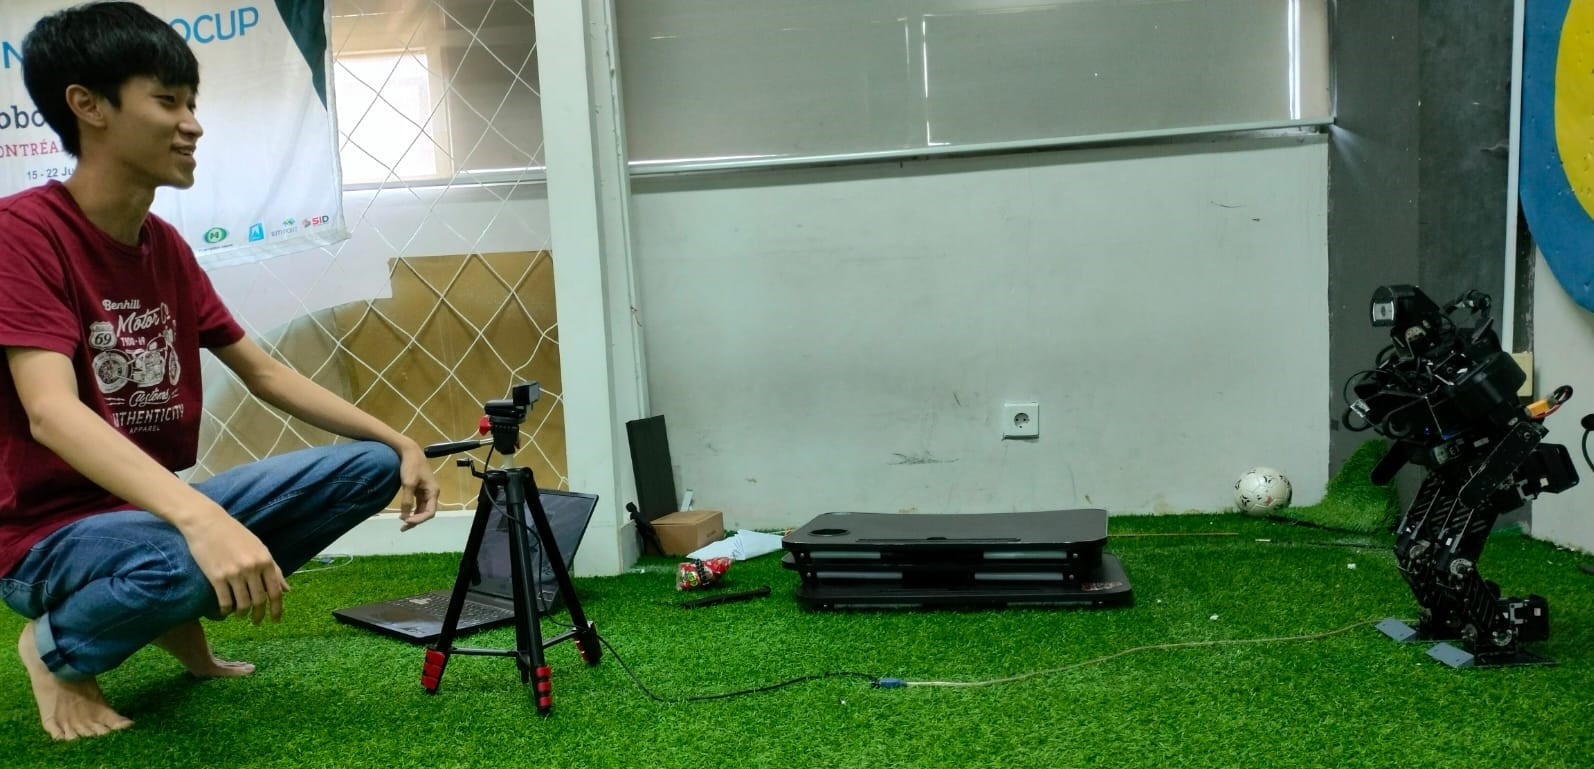
\includegraphics[width=0.47\textwidth]{gambar/pose-comparison.jpeg}
  \caption{Pose Comparison from Side.}
  \label{fig:pose-comparison-side}
\end{figure}

Since there are not many pose estimation models for humanoid robots out there yet, we need to retrain them or use transfer learning.
Therefore, the three following sections will explain about the steps for training pose estimation on humanoid robot.

\subsection{Make New Dataset}
\label{subsec:make-new-dataset}

This new dataset is a combination of NimbRo's HumanoidRobotPose dataset \citep{amini2021} and author own dataset. NimbRo's dataset contains both single and multiple robots with size teen and adult.
Overall, their dataset has over 1.5k images \citep{amini2021}.
However, the robots in Ichiro's dataset are only kid-sized and come in single or maximum two-robot configurations. The images in our dataset come from videos that are taken in our lab. 
Then we split up those videos into multiple images and pick not blurred one.
The newly created dataset has approximately 2.1k images, about 20 percent of the dataset was used for scoring and validating. We choose coco-annotator as our annotation tool. There are six keypoints including head, trunk, hands, and feet.


\subsection{Training Pose Estimation Model for Humanoid Robot}
\label{subsec:training-robot}

All of the training processes in this study were primarily conducted on a DGX-A100 server computer and written in the Python programing language.

\subsubsection{NimbRo's Model}
\label{subsubsec:training-nimbro-model}

The hyperparameters that are used to train NimbRo's model followed the description in their paper.
This model is trained using the AdamW optimizer with a learning rate of 10\textsuperscript{-4},
batch size 16, and weight decay of 10\textsuperscript{-4} for the total 200 epochs.
We also use data augmentation that includes random scaling and random translation \citep{amini2021}.
We do not use random horizontal flip and random rotation because in our case it will make the training result worse.


\subsubsection{YOLO-pose}
\label{subsubsec:training-yolo-pose}

Before we jumped into training process, the format change in our new dataset is needed from COCO to YOLO. They differ in defining visibility flags and bounding-box format.
The hyperparameters to train YOLO-pose followed the description in their GitHub named \emph{hyp.pose.yaml} .
We use SGD optimizer with a cosine scheduler. The base learning rate is set to 10\textsuperscript{-2}, batch size 16,
and weight decay of 5\textsuperscript{-4} for total 100 epochs. There are also data augmentation like random scale,
random translation, mosaic augmentation, and various color augmentations \citep{maji2022yolopose}.


\subsubsection{Keypoint RCNN}
\label{subsubsec:training-rcnn}

The Keypoint RCNN training is done on Jupyter Notebook directly using the PyTorch framework.
The training process starts with loading our dataset and specifying the augmentation technique like random brightness, contrast, and rotation using \emph{albumentations} library.
Before we declare Keypoint RCNN model using \emph{torchvision} library, we need anchors that will be an input argument. 
By default, the \emph{AnchorGenerator} class in PyTorch has 3 different \verb|sizes| (128, 256, 512) and 3 different \verb|aspect_ratios| (0.5, 1.0, 2.0).
We have extended those parameters, \verb|sizes| to (32, 64, 128, 256, 512) and \verb|aspect_ratios| to (0.25, 0.5, 0.75, 1.0, 2.0, 3.0, 4.0).
Note that, \verb|num classes| argument is set to two because the first class is background and object is the second class.
In this training, we use SGD optimizer with learning rate 10\textsuperscript{-3}, batch size 3, and weight decay of 5\textsuperscript{-4} for 50 epochs.


\subsection{Finding the Best Model for Humanoid Robot Pose Estimation}
\label{subsec:finding-best-model-humanoid-robot}

After retraining 3 models on Subsection \ref{subsec:training-robot}, we try to find the best one for our case. We compare them based on \emph{AP} (Average Precision), \emph{AR} (Average Recall),
real detection result, and inference time on devices with limited computing capabilities (e.g. NUC i5).
The comparison table and real detection result of those models are in Section \ref{sec:result-and-discussion}.
To know the time that it takes for the model to do the detection, we subtract the time before and after the model does keypoint detection.
We also attempt converting our models from PyTorch Model to OpenVINO in order to speed up the time inference.

\subsection{Choose Six Keypoints based on Humanoid Robot Keypoints}
\label{subsec:choose-keypoints}

The difference in numbers between human keypoints and robot keypoints makes us have to choose certain human's keypoints in order to make a comparison between them.
Based on the results after testing, we chose Mediapipe for human and Keypoint RCNN for robot. Mediapipe provides 33 landmark keypoints for human and Keypoint RCNN only provides 6 keypoints.
Therefore, we need to choose 6 from 33 human keypoint where the head keypoint is located between eyes, hands and feet keypoints is simply to select the wrists and ankles, also the trunk keypoint is located between the shoulder and hip keypoint.


\subsection{Keypoint Normalization}
\label{subsec:keypoint-normalization}

When we think about the problem, we see that there are many uncertainties to be addressed. For example, human and humanoid robot can differ in height, body shape, and location within an image: one subject (human or robot) may have been nearby the camera,
while another may have been in the distance. In order to get an accurate outcome, each of these issues must be resolved.
After choosing the keypoints, we create a new bounding box which tightly covers the object in the image.
This solves the problem of the subject appearing in different parts of the picture.
We further normalized the resulting keypoints coordinates by performing L2 normalization in order to transform it into a unit vector.
This means we are ignoring the size of the picture, but keeping in account the direction of the vector, created by the pose inside of that image.


\subsection{Comparing Human Keypoints and Robot Keypoints}
\label{subsec:comparing-keypoints}

Now that we have standardized the pose vectors, it is time to choose a similarity measure. We chose cosine similarity and performing a few calculations detailed below to arrive at a Euclidean distance that can be interpreted as a cosine distance.
The cosine similarity ranges from -1 to 1. The cosine distance, on the other hand, is a dissimilarity measure that ranges from 0 to 2.
Using Equation \ref{eq:euclideandistance} scales the values to the range of 0 to 2, making it easier to interpret the results. A larger value implies a greater dissimilarity between poses. In that equation, Fxy and Gxy are two pose vectors to be compared after L2 normalization. Moreover, Fxy and Gxy contain only x and y positions for each of the 6 keypoints, it does not include confidence scores.
\begin{equation} 
  \label{eq:cosinesimilarity}
  cosineSimilarity(x,y) = \frac{x \cdot y}{|x||y|}
\end{equation}

\begin{equation}
  \label{eq:euclideandistance}
  D(F_{xy}, G_{xy}) = \sqrt{2 * (1 - cosineSimilarity(F_{xy}, G_{xy}))}
\end{equation}


\subsection{Pose Similarity Result}
\label{subsec:pose-similarity-result}

The result of pose similarity is in percentages with a range of 0 to 100. A higher score indicates a more similar position between the human and robot, and vice versa.
In order to get it, we multiply the cosine distance result from Section \ref{subsec:comparing-keypoints} by 100 and subtract the result from 100.
After getting each result of pose similarity, we take a mean and display it in the left top video. This video will be generated after detecting and comparing all poses.
  % Ubah judul dan label berikut sesuai dengan yang diinginkan.
\section{Kesimpulan}
\label{sec:kesimpulan}

% Ubah paragraf-paragraf pada bagian ini sesuai dengan yang diinginkan.

\lipsum[21-23]


  % Menampilkan daftar pustaka dengan format IEEE
  \bibliographystyle{IEEEtranN}
  \bibliography{pustaka/pustaka.bib}

  % Menyeimbangkan bagian akhir di kedua kolom
  \balance

\end{document}
